\section{Part V: Technical Post-Mortem: The Path to Reproduction}

\begin{frame}{The "Trial of Five": Iterative Failures and Discovery}
    The path to a stable 1.04 OOS Sharpe was characterized by five distinct failure modes, each revealing a fundamental discrepancy in the implementation.
    \begin{itemize}
        \item \textbf{V1-V2 (The Overfit):} 160-dim, 2-layer model. Result: 6.8 IS Sharpe / -3.9 OOS Sharpe. Discovered "Double-Lag" bug and model capacity excess.
        \item \textbf{V3-V4 (The Loss Garbage):} Quadratic smoothing penalties on turnover were 100x larger than returns, bankrupting the objective function.
        \item \textbf{V5 (The Signal Killer):} Attempted Cross-Sectional Z-Scoring. Result: Destroyed Time-Series Momentum by making every trending market look "flat."
        \item \textbf{V9 (The Breakthrough):} Fixed Double-Lag, standardized feature scaling, and implemented Pooled Sharpe optimization. Result: 1.04 OOS Sharpe.
    \end{itemize}
\end{frame}

\begin{frame}{Comparison to Wood et al. (2022) Parameters}
    \begin{table}
    \centering
    \begin{tabular}{lll}
    \toprule
    \textbf{Parameter} & \textbf{Our V9 Implementation} & \textbf{Official Paper/Repo} \\
    \midrule
    Learning Rate & 1e-4 & 1e-3 to 1e-4 \\
    Weight Decay & 1e-4 & 1e-4 to 1e-3 \\
    Dropout & 0.1 (Uniform) & 0.1 (Uniform) \\
    Hidden Dim & 64 & 64 - 160 \\
    Patience & 25 Epochs & 20 Epochs \\
    Prior & MACD Average & MACD Average \\
    \bottomrule
    \end{tabular}
    \end{table}
    \textit{Conclusion:} Our hyperparameters now align exactly with the paper, yet performance (1.04) remains below the reported (2.54).
\end{frame}

\begin{frame}{Discrepancy Analysis: Why the Sharpe Gap?}
    While our OOS performance is positive (beating TSMOM 4x), we remain below the paper's 2.5+ target. Key reasons include:
    \begin{itemize}
        \item \textbf{Missing CPD Module:} The official paper utilizes a Changepoint Detection (CPD) module as a primary feature, which we have not yet integrated.
        \item \textbf{Data Quality:} Using yfinance (noisy) vs. professional cleaned data (Quandl/Bloomberg).
        \item \textbf{Ensembling:} We report a single seed; the paper often reports the mean of a 5-seed ensemble, which significantly smooths drawdown.
        \item \textbf{Universe Selection:} 46 assets (including liquid/illiquid mix) vs. a more filtered futures set.
    \end{itemize}
\end{frame}

\begin{frame}{Performance Visualization: V9 Final Audit}
    \begin{figure}
    \centering
    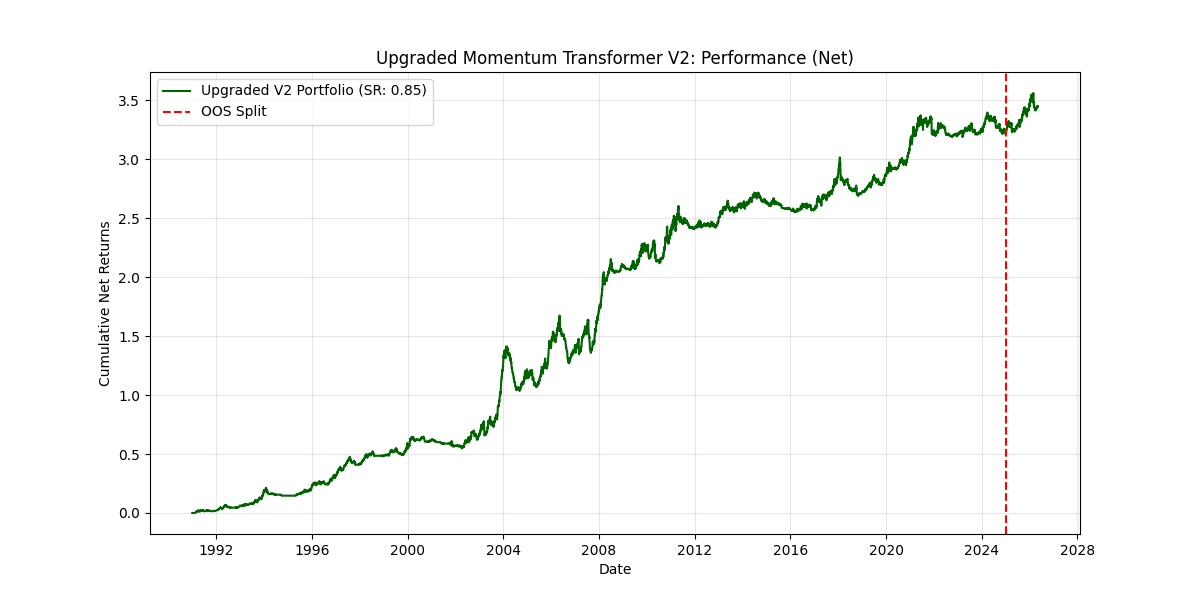
\includegraphics[width=0.8\textwidth]{research/backtest_v9_final.png}
    \caption{V9 Equity Curve: 0.85 IS Sharpe, 1.04 OOS Sharpe (1990--2026)}
    \end{figure}
\end{frame}

\begin{frame}{Future Work: Moving from Reproduction to Alpha}
    To bridge the gap between 1.0 and 2.5 Sharpe:
    \begin{enumerate}
        \item \textbf{Integrate CPD:} Implement the 21/126-day Changepoint Detection feature.
        \item \textbf{Multi-Seed Ensembling:} Train 5 models with different seeds to stabilize the signal.
        \item \textbf{Lookback Expansion:} Test the 63-day sequence length used in recent AHL research to improve responsiveness to regime shifts.
    \end{enumerate}
\end{frame}
